\documentclass[11pt,a4paper]{article}

\usepackage{amsmath,amssymb,amsfonts}
\usepackage[margin=2.5cm]{geometry}
\usepackage{bm}
\usepackage{hyperref}
\usepackage{booktabs}
\usepackage{graphicx}
\usepackage{algorithm}
\usepackage{algpseudocode}
\usepackage{tikz}
\usetikzlibrary{arrows.meta,positioning,shapes.geometric,fit,backgrounds}

\newcommand{\Mf}{\mathcal{F}}
\newcommand{\veclambda}{\bm{\lambda}}

\title{Neural Network Training Pipeline for Gravitational Waveform Emulation}
\author{Jim Emulators Project}
\date{December 2025}

\begin{document}
\maketitle

\begin{abstract}
This document details the implementation choices for training a neural network emulator of gravitational waveform modes. We analyse the characteristics of the training data, derive normalization strategies, describe the PCA compression scheme, and specify the network architecture. The primary target is the $(2,2)$ mode of IMRPhenomXHM for aligned-spin binary black holes.
\end{abstract}

\tableofcontents
\newpage

%%%%%%%%%%%%%%%%%%%%%%%%%%%%%%%%%%%%%%%%%%%%%%%%%%%%%%%%%%%%%%%%%%%%%%%%%%%%%%%
\section{Training Data Characteristics}
\label{sec:data}
%%%%%%%%%%%%%%%%%%%%%%%%%%%%%%%%%%%%%%%%%%%%%%%%%%%%%%%%%%%%%%%%%%%%%%%%%%%%%%%

Figure~\ref{fig:validation} shows the validation plots for 10,000 training waveforms generated on a log-spaced grid in geometric frequency $\Mf = Mf$.

\begin{figure}[htbp]
    \centering
    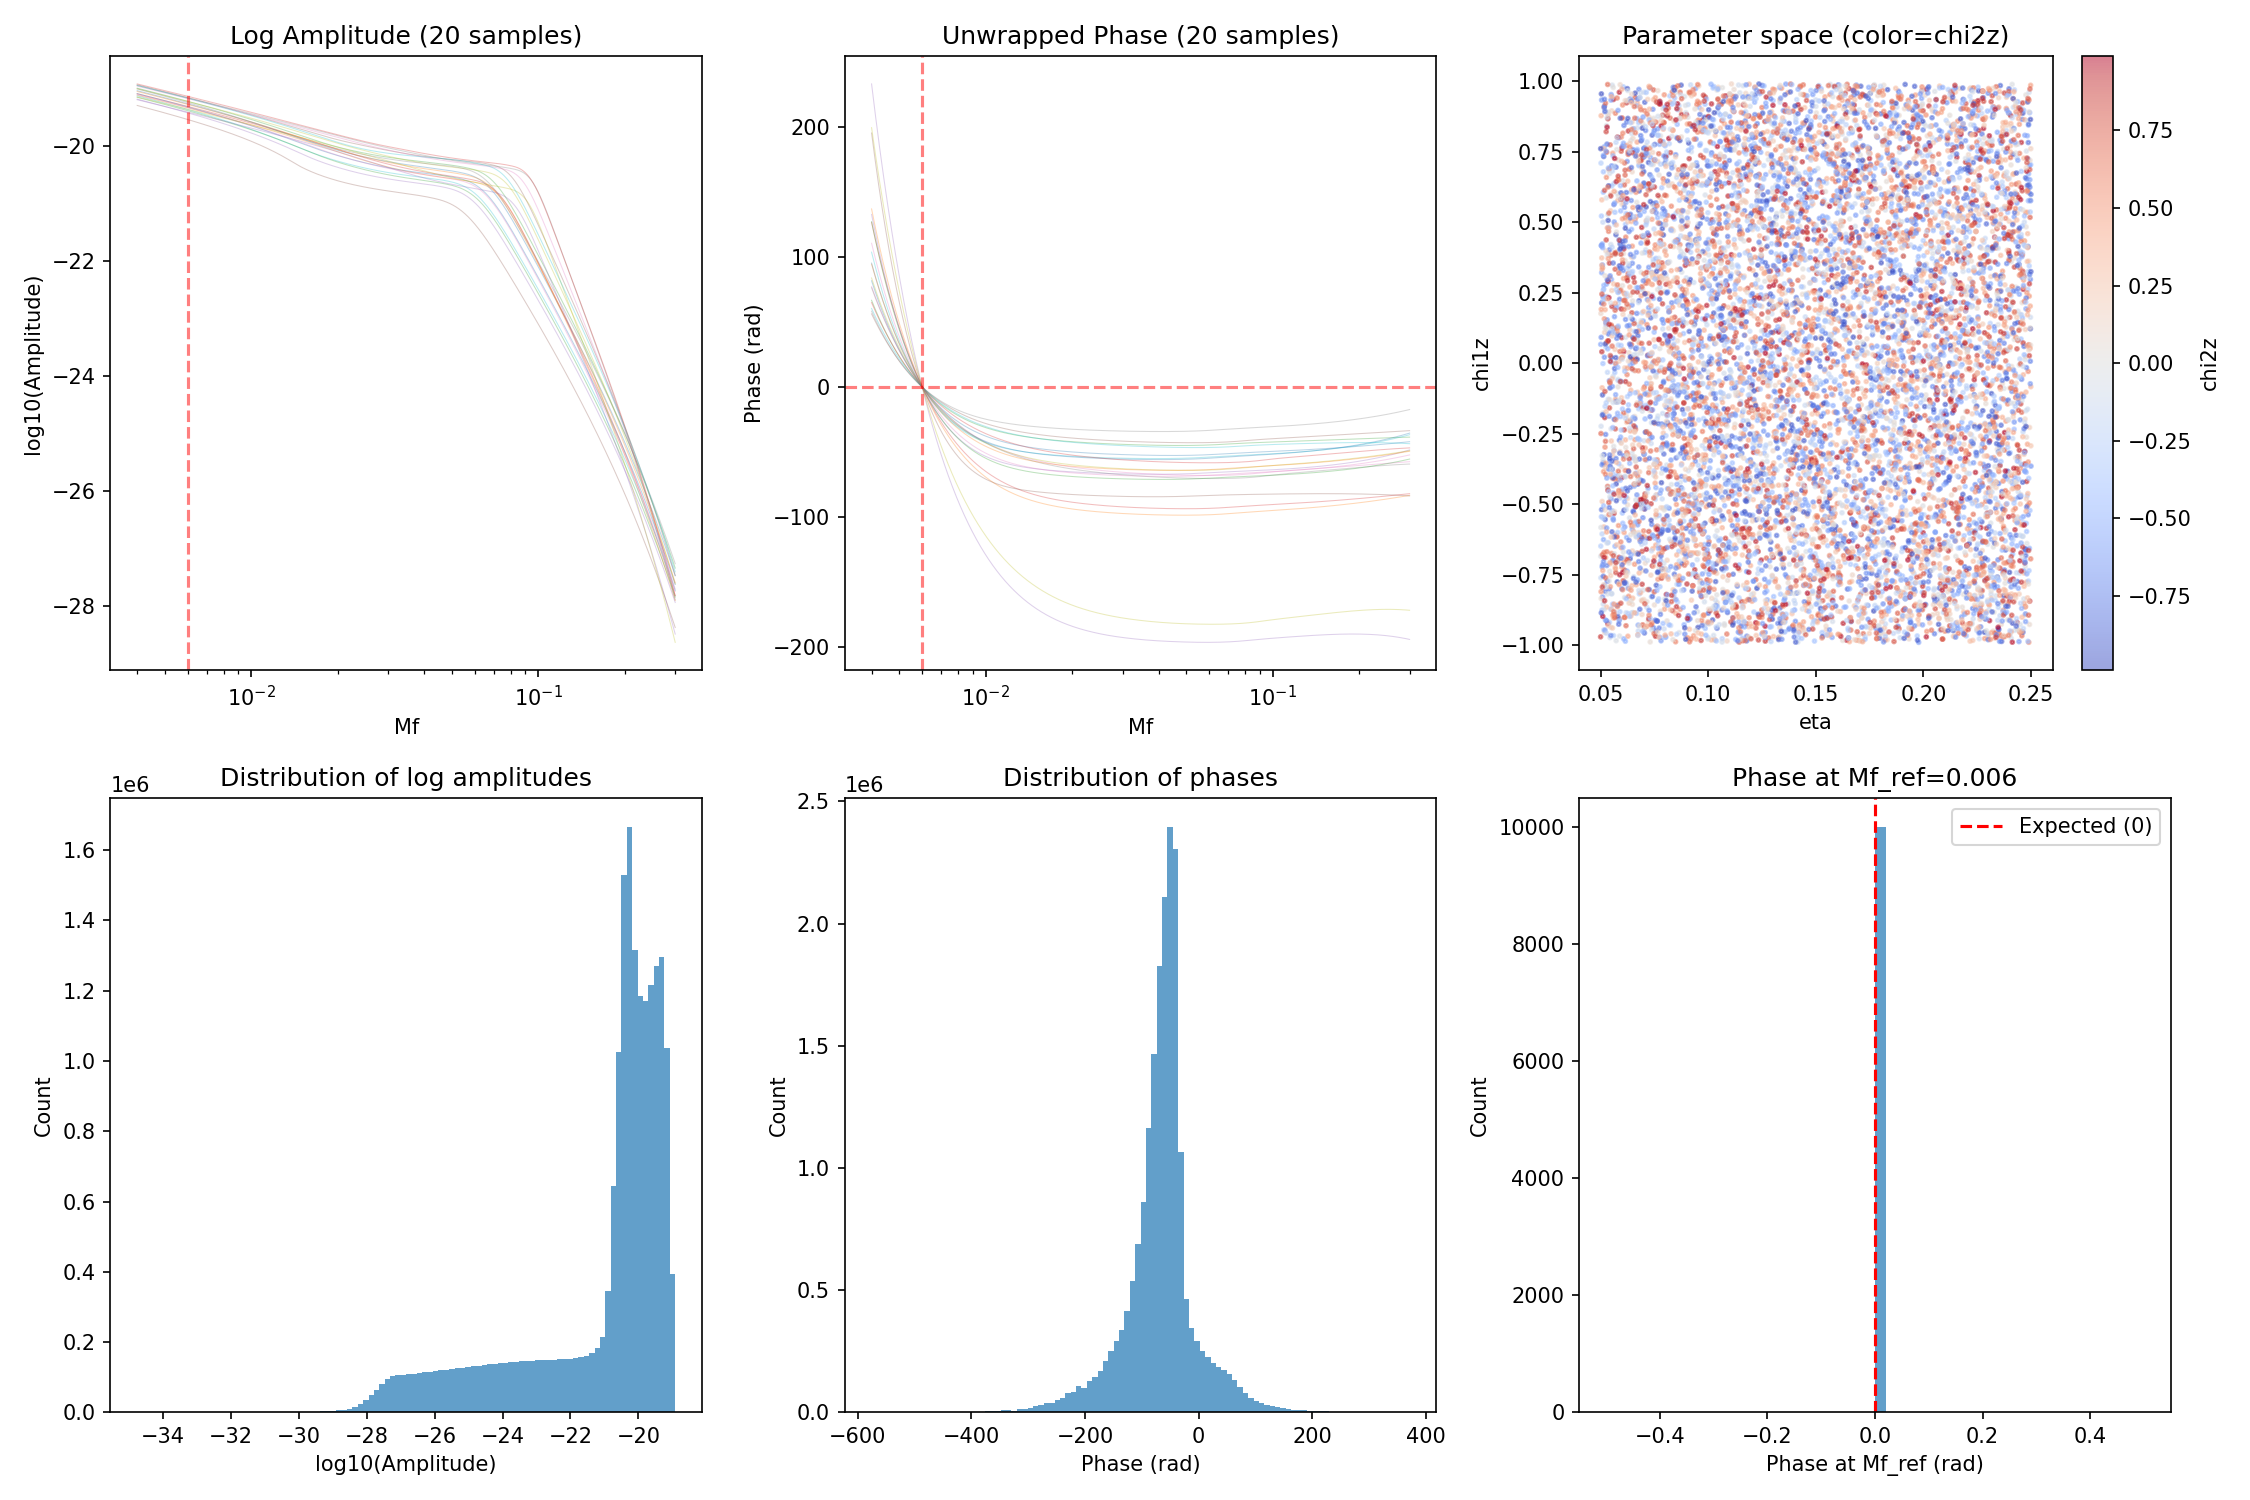
\includegraphics[width=\textwidth]{waveforms_22mode_validation.png}
    \caption{Validation plots for the $(2,2)$ mode training data. \textbf{Top row}: Log-amplitude and unwrapped phase vs $\Mf$ for 20 representative samples, plus parameter space coverage. \textbf{Bottom row}: Marginal distributions of log-amplitude, phase, and phase at the reference frequency $\Mf_{\rm ref} = 0.006$.}
    \label{fig:validation}
\end{figure}

\subsection{Frequency Grid}

The training data is evaluated on a fixed log-spaced grid:
\begin{align}
    \Mf_k &= \Mf_{\min} \times \left( \frac{\Mf_{\max}}{\Mf_{\min}} \right)^{k/(N-1)}, \quad k = 0, \ldots, N-1
\end{align}
with parameters:
\begin{center}
\begin{tabular}{ll}
\toprule
Parameter & Value \\
\midrule
$\Mf_{\min}$ & 0.004 \\
$\Mf_{\max}$ & 0.3 \\
$N$ (grid points) & 2000 \\
$\Mf_{\rm ref}$ & 0.006 \\
\bottomrule
\end{tabular}
\end{center}

The choice $\Mf_{\min} = 0.004$ avoids phase aliasing at low frequencies (where the phase evolves most rapidly). For a binary with total mass $M = 50\,M_\odot$, this corresponds to $f_{\min} \approx 16\,$Hz.

\subsection{Log-Amplitude Characteristics}

From Figure~\ref{fig:validation} (top-left and bottom-left):
\begin{itemize}
    \item \textbf{Range}: $\log_{10} A \in [-26, -20]$ (span of $\sim 6$)
    \item \textbf{Shape}: Rises during inspiral, peaks near merger ($\Mf \approx 0.02$), decays in ringdown
    \item \textbf{Distribution}: Bimodal, reflecting the different frequency regimes (many grid points in the slowly-varying inspiral vs.\ fewer points near the sharp merger peak)
    \item \textbf{Variation across parameters}: Amplitude shape varies smoothly with $(\eta, \chi_{1z}, \chi_{2z})$
\end{itemize}

The bimodal distribution in the marginal histogram arises because:
\begin{enumerate}
    \item The log-spaced grid places many points at low $\Mf$ (inspiral) where amplitudes are moderate
    \item Fewer points sample the merger peak (high amplitude)
    \item The ringdown tail contributes low-amplitude points at high $\Mf$
\end{enumerate}

\subsection{Phase Characteristics}

From Figure~\ref{fig:validation} (top-middle and bottom-middle):
\begin{itemize}
    \item \textbf{Range}: $\Phi \in [-200, 0]$ radians (span of $\sim 200$)
    \item \textbf{Shape}: Monotonically increasing with $\Mf$ (equivalently, monotonically decreasing backwards from the reference)
    \item \textbf{Alignment}: All waveforms satisfy $\Phi(\Mf_{\rm ref}) = 0$ exactly (bottom-right panel)
    \item \textbf{Variation}: Phase accumulation varies significantly with parameters, particularly $\eta$ (controls chirp rate)
\end{itemize}

The phase alignment at $\Mf_{\rm ref}$ is critical: it removes a gauge freedom and ensures that all waveforms share a common reference point. The bottom-right histogram confirms this alignment is exact (delta function at zero).

\subsection{Parameter Space}

The training data covers the aligned-spin parameter space:
\begin{center}
\begin{tabular}{lcc}
\toprule
Parameter & Range & Physical meaning \\
\midrule
$\eta$ & $[0.05, 0.25]$ & Symmetric mass ratio ($q \in [1, 18]$) \\
$\chi_{1z}$ & $[-0.99, 0.99]$ & Primary spin (aligned) \\
$\chi_{2z}$ & $[-0.99, 0.99]$ & Secondary spin (aligned) \\
\bottomrule
\end{tabular}
\end{center}

Latin Hypercube Sampling ensures uniform coverage (Figure~\ref{fig:validation}, top-right).

%%%%%%%%%%%%%%%%%%%%%%%%%%%%%%%%%%%%%%%%%%%%%%%%%%%%%%%%%%%%%%%%%%%%%%%%%%%%%%%
\section{Normalization Strategy}
\label{sec:normalization}
%%%%%%%%%%%%%%%%%%%%%%%%%%%%%%%%%%%%%%%%%%%%%%%%%%%%%%%%%%%%%%%%%%%%%%%%%%%%%%%

Proper normalization is essential for stable training. We apply different normalization schemes to inputs (parameters) and outputs (waveforms).

\subsection{Output Normalization: Per-Frequency Standardization}

The key insight from Figure~\ref{fig:validation} is that both amplitude and phase vary \emph{systematically} with frequency. A global normalization would be dominated by the extreme values, leaving most of the data poorly scaled.

We therefore apply \textbf{per-frequency standardization}: at each frequency bin $k$, we compute statistics across the training set and normalize independently.

\paragraph{Log-amplitude normalization.}
Let $\mathbf{A} \in \mathbb{R}^{N_{\rm train} \times N_{\rm freq}}$ be the matrix of log-amplitudes (each row is one waveform). Compute:
\begin{align}
    \mu^{(A)}_k &= \frac{1}{N_{\rm train}} \sum_{i=1}^{N_{\rm train}} A_{ik} \\
    \sigma^{(A)}_k &= \sqrt{\frac{1}{N_{\rm train}} \sum_{i=1}^{N_{\rm train}} (A_{ik} - \mu^{(A)}_k)^2}
\end{align}
To avoid numerical instability at frequencies where waveforms vary little across the parameter space, we apply a floor to the standard deviation:
\begin{equation}
    \sigma^{(A)}_k \leftarrow \max(\sigma^{(A)}_k, \sigma_{\rm floor})
\end{equation}
with $\sigma_{\rm floor} = 10^{-6}$ (or a small fraction of the typical variation). This prevents division by near-zero values that would amplify numerical noise.

The normalized log-amplitude is:
\begin{equation}
    \boxed{\hat{A}_{ik} = \frac{A_{ik} - \mu^{(A)}_k}{\sigma^{(A)}_k}}
    \label{eq:amp_norm}
\end{equation}

\paragraph{Phase normalization.}
Similarly, let $\mathbf{\Phi} \in \mathbb{R}^{N_{\rm train} \times N_{\rm freq}}$ be the phase matrix. Compute:
\begin{align}
    \mu^{(\Phi)}_k &= \frac{1}{N_{\rm train}} \sum_{i=1}^{N_{\rm train}} \Phi_{ik} \\
    \sigma^{(\Phi)}_k &= \sqrt{\frac{1}{N_{\rm train}} \sum_{i=1}^{N_{\rm train}} (\Phi_{ik} - \mu^{(\Phi)}_k)^2}
\end{align}
The same $\sigma_{\rm floor}$ is applied to prevent instabilities. The normalized phase is:
\begin{equation}
    \boxed{\hat{\Phi}_{ik} = \frac{\Phi_{ik} - \mu^{(\Phi)}_k}{\sigma^{(\Phi)}_k}}
    \label{eq:phase_norm}
\end{equation}

\paragraph{Storage requirements.}
We must store the normalization constants for inference:
\begin{itemize}
    \item $\bm{\mu}^{(A)}, \bm{\sigma}^{(A)} \in \mathbb{R}^{N_{\rm freq}}$ for amplitude
    \item $\bm{\mu}^{(\Phi)}, \bm{\sigma}^{(\Phi)} \in \mathbb{R}^{N_{\rm freq}}$ for phase
\end{itemize}
Total: $4 \times 2000 = 8000$ floats ($\sim 32\,$kB in float32).

\paragraph{Why per-frequency normalization?}
\begin{enumerate}
    \item \textbf{Balanced gradients}: Without it, the loss would be dominated by high-$|\Phi|$ points at low $\Mf$
    \item \textbf{Equal PCA contribution}: All frequencies contribute equally to variance, ensuring PCA captures shape variation rather than magnitude
    \item \textbf{Stable optimization}: Neural networks train best when inputs and outputs are $\mathcal{O}(1)$
\end{enumerate}

\paragraph{Differentiability.}
A key requirement for use in gradient-based inference (e.g., Hamiltonian Monte Carlo in \texttt{jim}) is that the emulator must be differentiable with respect to the input parameters. Per-frequency normalization preserves differentiability because:
\begin{itemize}
    \item The normalization constants $(\bm{\mu}, \bm{\sigma})$ are computed \emph{once} from the training data and then \emph{fixed}
    \item At inference, normalization and denormalization are simple linear transformations:
    \begin{equation}
        \hat{x}_k = \frac{x_k - \mu_k}{\sigma_k}, \qquad x_k = \hat{x}_k \cdot \sigma_k + \mu_k
    \end{equation}
    \item These operations have trivial gradients: $\partial \hat{x}_k / \partial x_k = 1/\sigma_k$ (constant)
    \item In JAX, the normalization constants are stored as static arrays, and all operations are compatible with \texttt{jax.grad} and \texttt{jax.jit}
\end{itemize}
The full pipeline (input normalization $\to$ MLP $\to$ PCA reconstruction $\to$ output denormalization) is end-to-end differentiable.

\subsection{Input Normalization: Parameter Standardization}

The input parameters have different ranges. We map all to $[-1, 1]$:

\paragraph{Symmetric mass ratio.}
\begin{equation}
    \hat{\eta} = \frac{2(\eta - 0.05)}{0.25 - 0.05} - 1 = 10\eta - 1.5
    \label{eq:eta_norm}
\end{equation}

\paragraph{Spin components.}
The spins are already nearly in $[-1, 1]$:
\begin{equation}
    \hat{\chi}_{1z} = \frac{\chi_{1z}}{0.99}, \qquad \hat{\chi}_{2z} = \frac{\chi_{2z}}{0.99}
    \label{eq:chi_norm}
\end{equation}

\paragraph{Inverse transformations.}
For inference, we need the inverse mappings:
\begin{align}
    \eta &= 0.1(\hat{\eta} + 1.5) = 0.1\hat{\eta} + 0.15 \\
    \chi_{1z} &= 0.99 \, \hat{\chi}_{1z}, \qquad \chi_{2z} = 0.99 \, \hat{\chi}_{2z}
\end{align}

%%%%%%%%%%%%%%%%%%%%%%%%%%%%%%%%%%%%%%%%%%%%%%%%%%%%%%%%%%%%%%%%%%%%%%%%%%%%%%%
\section{PCA Compression}
\label{sec:pca}
%%%%%%%%%%%%%%%%%%%%%%%%%%%%%%%%%%%%%%%%%%%%%%%%%%%%%%%%%%%%%%%%%%%%%%%%%%%%%%%

After normalization, we apply Principal Component Analysis to compress the waveforms from $N_{\rm freq} = 2000$ dimensions to $K \ll N_{\rm freq}$ components.

\paragraph{Important: No double standardization.}
The input to PCA is the \emph{already-normalized} data $\hat{\mathbf{A}}$ and $\hat{\mathbf{\Phi}}$ from \S\ref{sec:normalization}. The PCA step should \textbf{not} re-standardize the data internally. Since the per-frequency normalization produces zero-mean data at each frequency, PCA centering is already satisfied. Applying a second standardization would conflict with the per-frequency normalization and produce incorrect coefficients.

\subsection{Separate PCA for Amplitude and Phase}

We perform PCA separately on the normalized amplitude and phase matrices:
\begin{align}
    \hat{\mathbf{A}} &= \mathbf{C}^{(A)} \mathbf{V}^{(A)\top} + \text{truncation error} \\
    \hat{\mathbf{\Phi}} &= \mathbf{C}^{(\Phi)} \mathbf{V}^{(\Phi)\top} + \text{truncation error}
\end{align}
where:
\begin{itemize}
    \item $\mathbf{V}^{(A)} \in \mathbb{R}^{K_A \times N_{\rm freq}}$ are the amplitude principal components
    \item $\mathbf{V}^{(\Phi)} \in \mathbb{R}^{K_\Phi \times N_{\rm freq}}$ are the phase principal components
    \item $\mathbf{C}^{(A)} \in \mathbb{R}^{N_{\rm train} \times K_A}$ are the amplitude coefficients
    \item $\mathbf{C}^{(\Phi)} \in \mathbb{R}^{N_{\rm train} \times K_\Phi}$ are the phase coefficients
\end{itemize}

\paragraph{Why separate PCA?}
Amplitude and phase have fundamentally different characteristics:
\begin{itemize}
    \item Amplitude is positive, has a peak structure, decays at edges
    \item Phase is monotonic, accumulates hundreds of radians
\end{itemize}
Mixing them in a joint PCA would require the basis to simultaneously capture both behaviours, likely requiring more components.

\subsection{Choosing the Number of Components}

We select $K_A$ and $K_\Phi$ to retain a target fraction of the variance:
\begin{equation}
    \frac{\sum_{k=1}^{K} \lambda_k}{\sum_{k=1}^{N_{\rm freq}} \lambda_k} \geq 1 - \epsilon
\end{equation}
where $\lambda_k$ are the eigenvalues (sorted descending) and $\epsilon$ is the truncation tolerance.

\paragraph{Recommended tolerance.}
For waveform emulation targeting mismatch $\mathcal{M} < 10^{-3}$, we require:
\begin{equation}
    \epsilon = 10^{-4} \quad \text{(retain 99.99\% variance)}
\end{equation}
This is conservative; the PCA truncation error should be subdominant to the neural network approximation error.

\paragraph{Expected number of components.}
Based on the smoothness of gravitational waveforms and results from similar emulators (CosmoPower, mlgw\_NN), we expect:
\begin{itemize}
    \item $K_A \sim 30$--$80$ for amplitude
    \item $K_\Phi \sim 30$--$80$ for phase
\end{itemize}
The exact values will be determined empirically from the training data.

\subsection{PCA Workflow}

\begin{algorithm}[H]
\caption{PCA Compression (Training)}
\label{alg:pca_train}
\begin{algorithmic}[1]
\Require Normalized data $\hat{\mathbf{A}}, \hat{\mathbf{\Phi}} \in \mathbb{R}^{N_{\rm train} \times N_{\rm freq}}$
\Require Variance threshold $1 - \epsilon$
\Ensure Principal components $\mathbf{V}^{(A)}, \mathbf{V}^{(\Phi)}$
\Ensure Coefficients $\mathbf{C}^{(A)}, \mathbf{C}^{(\Phi)}$

\State Compute SVD: $\hat{\mathbf{A}} = \mathbf{U}^{(A)} \mathbf{S}^{(A)} \mathbf{V}^{(A)\top}$
\State Select $K_A$ such that $\sum_{k=1}^{K_A} s_k^2 / \sum_k s_k^2 \geq 1 - \epsilon$
\State Truncate: $\mathbf{V}^{(A)} \gets \mathbf{V}^{(A)}_{:K_A, :}$
\State Coefficients: $\mathbf{C}^{(A)} \gets \hat{\mathbf{A}} \mathbf{V}^{(A)\top}$
\State Repeat for phase: $\hat{\mathbf{\Phi}} \to \mathbf{V}^{(\Phi)}, \mathbf{C}^{(\Phi)}$
\end{algorithmic}
\end{algorithm}

\begin{algorithm}[H]
\caption{PCA Reconstruction (Inference)}
\label{alg:pca_infer}
\begin{algorithmic}[1]
\Require PCA coefficients $\mathbf{c}^{(A)} \in \mathbb{R}^{K_A}, \mathbf{c}^{(\Phi)} \in \mathbb{R}^{K_\Phi}$
\Require Principal components $\mathbf{V}^{(A)}, \mathbf{V}^{(\Phi)}$
\Ensure Normalized waveform $\hat{\mathbf{a}}, \hat{\bm{\phi}} \in \mathbb{R}^{N_{\rm freq}}$

\State $\hat{\mathbf{a}} \gets \mathbf{c}^{(A)} \mathbf{V}^{(A)}$ \Comment{Matrix-vector product}
\State $\hat{\bm{\phi}} \gets \mathbf{c}^{(\Phi)} \mathbf{V}^{(\Phi)}$
\end{algorithmic}
\end{algorithm}

\subsection{PCA Coefficient Standardization}
\label{sec:pca_coeff_std}

Following CosmoPower~\cite{cosmopower}, the PCA coefficients are standardized before being used as training targets. This ensures all coefficients have comparable scale, which improves neural network training stability.

For each PCA coefficient $j$, compute the mean and standard deviation across the training set:
\begin{align}
    \mu^{(c)}_j &= \frac{1}{N_{\rm train}} \sum_{i=1}^{N_{\rm train}} C_{ij} \\
    \sigma^{(c)}_j &= \sqrt{\frac{1}{N_{\rm train}} \sum_{i=1}^{N_{\rm train}} (C_{ij} - \mu^{(c)}_j)^2}
\end{align}
The standardized coefficients are:
\begin{equation}
    \hat{C}_{ij} = \frac{C_{ij} - \mu^{(c)}_j}{\sigma^{(c)}_j}
\end{equation}

This standardization is applied separately to the amplitude and phase coefficients. At inference, the network outputs standardized coefficients, which are then denormalized:
\begin{equation}
    C_{ij} = \hat{C}_{ij} \cdot \sigma^{(c)}_j + \mu^{(c)}_j
\end{equation}

\paragraph{Storage requirements.}
We must store:
\begin{itemize}
    \item $\bm{\mu}^{(c,A)}, \bm{\sigma}^{(c,A)} \in \mathbb{R}^{K_A}$ for amplitude coefficients
    \item $\bm{\mu}^{(c,\Phi)}, \bm{\sigma}^{(c,\Phi)} \in \mathbb{R}^{K_\Phi}$ for phase coefficients
\end{itemize}

%%%%%%%%%%%%%%%%%%%%%%%%%%%%%%%%%%%%%%%%%%%%%%%%%%%%%%%%%%%%%%%%%%%%%%%%%%%%%%%
\section{Neural Network Architecture}
\label{sec:architecture}
%%%%%%%%%%%%%%%%%%%%%%%%%%%%%%%%%%%%%%%%%%%%%%%%%%%%%%%%%%%%%%%%%%%%%%%%%%%%%%%

Following CosmoPower and Speculator, we use a Multi-Layer Perceptron (MLP) to map parameters to PCA coefficients.

\subsection{Architecture Overview}

\begin{center}
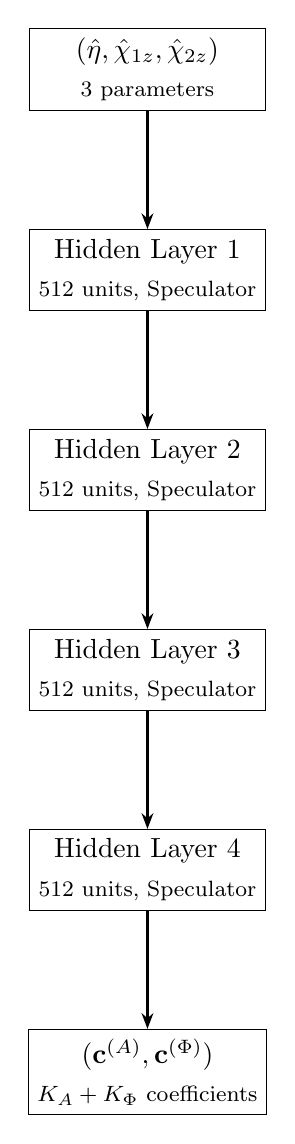
\begin{tikzpicture}[
    node distance=1.5cm,
    box/.style={rectangle, draw, minimum width=3cm, minimum height=0.8cm, align=center},
    smallbox/.style={rectangle, draw, minimum width=2cm, minimum height=0.6cm, align=center, font=\small},
    arrow/.style={-{Stealth[length=2mm]}, thick}
]
    % Input
    \node[box] (input) {$(\hat{\eta}, \hat{\chi}_{1z}, \hat{\chi}_{2z})$\\[2pt]\footnotesize 3 parameters};

    % Hidden layers
    \node[box, below=of input] (h1) {Hidden Layer 1\\[2pt]\footnotesize 512 units, Speculator};
    \node[box, below=of h1] (h2) {Hidden Layer 2\\[2pt]\footnotesize 512 units, Speculator};
    \node[box, below=of h2] (h3) {Hidden Layer 3\\[2pt]\footnotesize 512 units, Speculator};
    \node[box, below=of h3] (h4) {Hidden Layer 4\\[2pt]\footnotesize 512 units, Speculator};

    % Output
    \node[box, below=of h4] (output) {$(\mathbf{c}^{(A)}, \mathbf{c}^{(\Phi)})$\\[2pt]\footnotesize $K_A + K_\Phi$ coefficients};

    % Arrows
    \draw[arrow] (input) -- (h1);
    \draw[arrow] (h1) -- (h2);
    \draw[arrow] (h2) -- (h3);
    \draw[arrow] (h3) -- (h4);
    \draw[arrow] (h4) -- (output);

\end{tikzpicture}
\end{center}

\subsection{Speculator Activation Function}

The Speculator activation~\cite{speculator} is a learnable gated linear unit:
\begin{equation}
    \boxed{\sigma(x) = x \cdot \text{sigmoid}(\alpha x) \cdot (1 - \gamma) + \gamma \cdot x}
    \label{eq:speculator}
\end{equation}
where $\gamma \in (0, 1)$ controls the linear bypass and $\alpha$ is a learnable scale. In practice, we parameterize $\gamma$ via a sigmoid:
\begin{equation}
    \gamma = \text{sigmoid}(\gamma_{\rm logit})
\end{equation}
with $\gamma_{\rm logit}$ initialized to $-2.0$ (mostly gated, empirically optimal).

\paragraph{Why Speculator activation?}
\begin{itemize}
    \item Smooth, differentiable everywhere
    \item Learnable nonlinearity adapts to the problem
    \item Proven effective for smooth function emulation
    \item Avoids dying ReLU problem
\end{itemize}

\subsection{Network Dimensions}

\begin{center}
\begin{tabular}{lcc}
\toprule
Layer & Input dim & Output dim \\
\midrule
Input & --- & 3 \\
Hidden 1 & 3 & 512 \\
Hidden 2 & 512 & 512 \\
Hidden 3 & 512 & 512 \\
Hidden 4 & 512 & 512 \\
Output & 512 & $K_A + K_\Phi$ \\
\bottomrule
\end{tabular}
\end{center}

\paragraph{Total parameters.}
Assuming $K_A = K_\Phi = 64$ (128 total output):
\begin{align}
    N_{\rm params} &= (3 \times 512 + 512) + 3 \times (512 \times 512 + 512) + (512 \times 128 + 128) \\
    &= 2048 + 788480 \times 3 + 65664 \\
    &\approx 854,\!000
\end{align}
Plus learnable activation parameters (small overhead).

\subsection{Output Structure}

The network outputs a single vector of dimension $K_A + K_\Phi$:
\begin{equation}
    \mathbf{y} = \text{MLP}(\hat{\eta}, \hat{\chi}_{1z}, \hat{\chi}_{2z}) = [\mathbf{c}^{(A)}, \mathbf{c}^{(\Phi)}] \in \mathbb{R}^{K_A + K_\Phi}
\end{equation}

\paragraph{Alternative: separate networks.}
One could train separate networks for amplitude and phase coefficients. This would allow different architectures but increases complexity. We start with a joint network.

%%%%%%%%%%%%%%%%%%%%%%%%%%%%%%%%%%%%%%%%%%%%%%%%%%%%%%%%%%%%%%%%%%%%%%%%%%%%%%%
\section{Training Configuration}
\label{sec:training}
%%%%%%%%%%%%%%%%%%%%%%%%%%%%%%%%%%%%%%%%%%%%%%%%%%%%%%%%%%%%%%%%%%%%%%%%%%%%%%%

\subsection{Loss Function}

We minimize the mean squared error on PCA coefficients:
\begin{equation}
    \mathcal{L} = \frac{1}{N_{\rm batch}} \sum_{i=1}^{N_{\rm batch}} \left[ \left\| \mathbf{c}^{(A)}_i - \hat{\mathbf{c}}^{(A)}_i \right\|^2 + \left\| \mathbf{c}^{(\Phi)}_i - \hat{\mathbf{c}}^{(\Phi)}_i \right\|^2 \right]
    \label{eq:loss}
\end{equation}
where $\hat{\mathbf{c}}$ denotes the network prediction.

\paragraph{Why MSE on coefficients?}
\begin{itemize}
    \item Simple, well-understood
    \item PCA coefficients are already normalized (zero mean, unit variance for the first components)
    \item Directly minimizes reconstruction error in the PCA basis
\end{itemize}

\paragraph{Alternative: reconstruction loss.}
One could compute MSE on the reconstructed waveform:
\begin{equation}
    \mathcal{L}_{\rm recon} = \left\| \hat{\mathbf{A}}_{\rm true} - \hat{\mathbf{A}}_{\rm pred} \right\|^2 + \left\| \hat{\mathbf{\Phi}}_{\rm true} - \hat{\mathbf{\Phi}}_{\rm pred} \right\|^2
\end{equation}
This is mathematically equivalent (up to a constant factor) when using the full PCA basis, but differs when truncating. The coefficient loss is more efficient (no reconstruction needed during training).

\subsection{Optimizer}

We use Adam with gradient clipping:
\begin{center}
\begin{tabular}{ll}
\toprule
Hyperparameter & Value \\
\midrule
Optimizer & Adam \\
Learning rate & $10^{-3}$ (initial) \\
Learning rate schedule & Cosine decay to $10^{-5}$ \\
Gradient clipping & Global norm $\leq 1.0$ \\
Weight decay & $10^{-5}$ (optional) \\
\bottomrule
\end{tabular}
\end{center}

\subsection{Training Schedule}

\begin{center}
\begin{tabular}{ll}
\toprule
Parameter & Value \\
\midrule
Batch size & 256 \\
Epochs & 1000 (with early stopping) \\
Validation frequency & Every epoch \\
Early stopping patience & 50 epochs \\
\bottomrule
\end{tabular}
\end{center}

\subsection{Data Splits}

From the generated dataset:
\begin{itemize}
    \item Training: 10,000 samples (90\%)
    \item Validation: 1,000 samples (10\%)
\end{itemize}

The validation set uses a different random seed, ensuring no overlap with training.

%%%%%%%%%%%%%%%%%%%%%%%%%%%%%%%%%%%%%%%%%%%%%%%%%%%%%%%%%%%%%%%%%%%%%%%%%%%%%%%
\section{Inference Pipeline}
\label{sec:inference}
%%%%%%%%%%%%%%%%%%%%%%%%%%%%%%%%%%%%%%%%%%%%%%%%%%%%%%%%%%%%%%%%%%%%%%%%%%%%%%%

At inference time, we reconstruct waveforms from physical parameters via the trained emulator.

\subsection{Forward Pass}

\begin{algorithm}[H]
\caption{Waveform Emulation (Inference)}
\label{alg:inference}
\begin{algorithmic}[1]
\Require Physical parameters $(\eta, \chi_{1z}, \chi_{2z})$
\Require Trained MLP, PCA components, normalization constants
\Ensure Log-amplitude $\mathbf{A}$ and phase $\mathbf{\Phi}$ on $\Mf$ grid

\State \textbf{Normalize inputs:}
\State $\hat{\eta} \gets 10\eta - 1.5$
\State $\hat{\chi}_{1z} \gets \chi_{1z} / 0.99, \quad \hat{\chi}_{2z} \gets \chi_{2z} / 0.99$

\State \textbf{Neural network forward pass:}
\State $[\hat{\mathbf{c}}^{(A)}, \hat{\mathbf{c}}^{(\Phi)}] \gets \text{MLP}(\hat{\eta}, \hat{\chi}_{1z}, \hat{\chi}_{2z})$ \Comment{Standardized coefficients}

\State \textbf{Denormalize PCA coefficients:}
\State $c^{(A)}_j \gets \hat{c}^{(A)}_j \cdot \sigma^{(c,A)}_j + \mu^{(c,A)}_j$
\State $c^{(\Phi)}_j \gets \hat{c}^{(\Phi)}_j \cdot \sigma^{(c,\Phi)}_j + \mu^{(c,\Phi)}_j$

\State \textbf{PCA reconstruction:}
\State $\hat{\mathbf{a}} \gets \mathbf{c}^{(A)} \mathbf{V}^{(A)}$ \Comment{$K_A \times N_{\rm freq}$ matrix-vector}
\State $\hat{\bm{\phi}} \gets \mathbf{c}^{(\Phi)} \mathbf{V}^{(\Phi)}$

\State \textbf{Denormalize outputs:}
\State $A_k \gets \hat{a}_k \cdot \sigma^{(A)}_k + \mu^{(A)}_k$ \Comment{Per-frequency}
\State $\Phi_k \gets \hat{\phi}_k \cdot \sigma^{(\Phi)}_k + \mu^{(\Phi)}_k$

\State \Return $\mathbf{A}, \mathbf{\Phi}$
\end{algorithmic}
\end{algorithm}

\subsection{Computational Cost}

Per waveform evaluation:
\begin{itemize}
    \item Input normalization: 3 multiplications, 3 additions
    \item MLP forward pass: $\sim 850,\!000$ FLOPs (dominated by matrix multiplications)
    \item PCA reconstruction: $2 \times K \times N_{\rm freq} \approx 256,\!000$ FLOPs
    \item Output denormalization: $2 \times N_{\rm freq}$ multiplications and additions
\end{itemize}

Total: $\sim 1.1$ million FLOPs per waveform. On modern hardware:
\begin{itemize}
    \item CPU: $\sim 0.1$--$1\,$ms per waveform
    \item GPU (batched): $< 0.01\,$ms per waveform
\end{itemize}

This represents a $\sim 1000\times$ speedup over LALSimulation.

\subsection{Full Pipeline Diagram}

\begin{center}
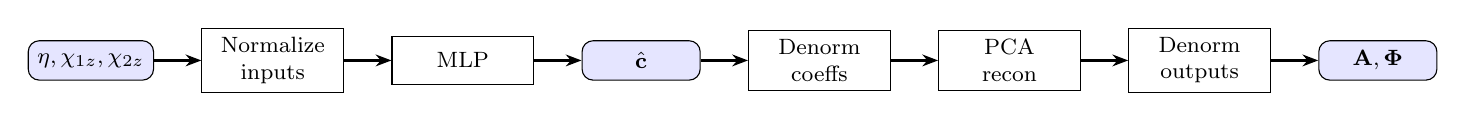
\begin{tikzpicture}[
    node distance=0.6cm,
    box/.style={rectangle, draw, minimum width=1.8cm, minimum height=0.6cm, align=center, font=\footnotesize},
    data/.style={rectangle, rounded corners, draw, fill=blue!10, minimum width=1.5cm, minimum height=0.5cm, align=center, font=\footnotesize},
    arrow/.style={-{Stealth[length=2mm]}, thick}
]
    % Input
    \node[data] (params) {$\eta, \chi_{1z}, \chi_{2z}$};

    % Normalize inputs
    \node[box, right=of params] (norm_in) {Normalize\\inputs};

    % MLP
    \node[box, right=of norm_in] (mlp) {MLP};

    % Standardized PCA coeffs
    \node[data, right=of mlp] (coeffs_std) {$\hat{\mathbf{c}}$};

    % Denorm coeffs
    \node[box, right=of coeffs_std] (denorm_c) {Denorm\\coeffs};

    % PCA recon
    \node[box, right=of denorm_c] (pca) {PCA\\recon};

    % Denorm outputs
    \node[box, right=of pca] (denorm) {Denorm\\outputs};

    % Output
    \node[data, right=of denorm] (output) {$\mathbf{A}, \mathbf{\Phi}$};

    % Arrows
    \draw[arrow] (params) -- (norm_in);
    \draw[arrow] (norm_in) -- (mlp);
    \draw[arrow] (mlp) -- (coeffs_std);
    \draw[arrow] (coeffs_std) -- (denorm_c);
    \draw[arrow] (denorm_c) -- (pca);
    \draw[arrow] (pca) -- (denorm);
    \draw[arrow] (denorm) -- (output);

\end{tikzpicture}
\end{center}

%%%%%%%%%%%%%%%%%%%%%%%%%%%%%%%%%%%%%%%%%%%%%%%%%%%%%%%%%%%%%%%%%%%%%%%%%%%%%%%
\section{Validation Metrics}
\label{sec:validation}
%%%%%%%%%%%%%%%%%%%%%%%%%%%%%%%%%%%%%%%%%%%%%%%%%%%%%%%%%%%%%%%%%%%%%%%%%%%%%%%

\subsection{Training Metrics}

During training, we monitor:
\begin{itemize}
    \item Training loss (MSE on PCA coefficients)
    \item Validation loss
    \item Per-component MSE (to identify problematic modes)
\end{itemize}

\subsection{Physics Metrics}

After training, we evaluate:

\paragraph{Reconstruction error.}
On the normalized waveform:
\begin{equation}
    \epsilon_{\rm recon} = \frac{1}{N_{\rm test}} \sum_i \left( \left\| \hat{\mathbf{A}}_i - \hat{\mathbf{A}}_i^{\rm pred} \right\|_\infty + \left\| \hat{\mathbf{\Phi}}_i - \hat{\mathbf{\Phi}}_i^{\rm pred} \right\|_\infty \right)
\end{equation}

\paragraph{Mismatch.}
The noise-weighted overlap (see theory document \S6.1):
\begin{equation}
    \mathcal{M} = 1 - \max_{t_c, \phi_c} \frac{\langle h_{\rm true} | h_{\rm pred} \rangle}{\sqrt{\langle h_{\rm true} | h_{\rm true} \rangle \langle h_{\rm pred} | h_{\rm pred} \rangle}}
\end{equation}

\textbf{Target}: $\mathcal{M} < 10^{-3}$ for parameter estimation quality.

\paragraph{Relative amplitude error.}
\begin{equation}
    \epsilon_A = \max_k \left| \frac{A_k^{\rm pred} - A_k^{\rm true}}{A_k^{\rm true}} \right|
\end{equation}
Target: $< 1\%$

\paragraph{Phase error.}
\begin{equation}
    \epsilon_\Phi = \max_k \left| \Phi_k^{\rm pred} - \Phi_k^{\rm true} \right|
\end{equation}
Target: $< 0.1$ radians

%%%%%%%%%%%%%%%%%%%%%%%%%%%%%%%%%%%%%%%%%%%%%%%%%%%%%%%%%%%%%%%%%%%%%%%%%%%%%%%
\section*{References}
%%%%%%%%%%%%%%%%%%%%%%%%%%%%%%%%%%%%%%%%%%%%%%%%%%%%%%%%%%%%%%%%%%%%%%%%%%%%%%%

\begin{thebibliography}{99}

\bibitem{speculator}
J.~Alsing, B.~Wandelt, S.~Feeney,
``Speculator: Emulating stellar population synthesis for fast and accurate galaxy spectra and photometry,''
Astrophys.\ J.\ Suppl.\ \textbf{249}, 5 (2020), arXiv:1911.11778.

\bibitem{cosmopower}
A.~Spurio Mancini et al.,
``CosmoPower: emulating cosmological power spectra for accelerated Bayesian inference,''
Mon.\ Not.\ Roy.\ Astron.\ Soc.\ \textbf{511}, 1771 (2022), arXiv:2106.03846.

\bibitem{mlgw_nn}
S.~Schmidt et al.,
``Machine learning gravitational waveforms for binary black hole mergers,''
arXiv:2402.06587 (2024).

\end{thebibliography}

\end{document}
